% !TeX spellcheck = pt_BR
\documentclass[12pt]{article}
\usepackage[margin=0.5in]{geometry}
\setlength{\parindent}{0pt} 
\setlength{\parskip}{5pt} 
\pagenumbering{gobble}
\setlength{\parindent}{10ex}

\usepackage[utf8]{inputenc}
\usepackage{amsmath,amsthm,amssymb}
\usepackage{graphicx}
\usepackage{float}
\usepackage[portuguese]{babel}


% TODO: Alterar a fonte das legendas e labels do gráfico
% TODO: Finalizar com qual o melhor caso para o boxplot

\title{PI IV - Visualização de dados numéricos}
\author{Lucas Gomes Santana}
\date{\today}

\begin{document}

\maketitle

Para as visualizações foi utilizado um subconjunto dos dados da tabela "Zonal annual means, 1880-present" disponibilizados pelo GISS Surface Temperature Analysis (GISTEMP v4)\cite{gistemp}, contendo números das alterações da média de temperatura global, do hemisfério sul e norte. Em ambos gráficos o eixo y representa a alteração da média de temperatura anual enquanto o eixo x representa o ano da alteração.\\


\textbf{\Large Gráfico de linhas}\par
A primeira representação dos dados numéricos é por meio de linhas.  Como os dados representam as alterações com o passar do tempo, um gráfico do tipo linha pode mostrar a progressão e tendências futuras.
\setcounter{figure}{0}
\begin{figure}[H]
\centering
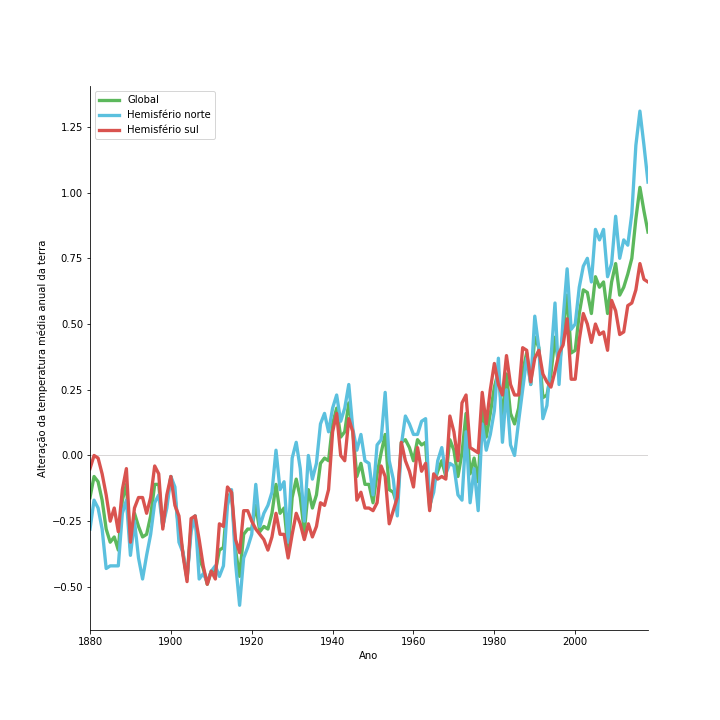
\includegraphics[width = 0.675\textwidth]{lines.png}
\label{fig:A.1}
\caption{Gráfico de linha mostrando a alteração de temperatura anual da terra pelo tempo.}
\end{figure}

\textbf{\Large Boxplot}\par
A segunda representação é do tipo 'boxplot'. Esse tipo de gráfico é usado para mostrar de forma rápida a distribuição dos dados, outliers e o quão simétricos eles são.
\setcounter{figure}{1}
\begin{figure}[H]
	\centering
	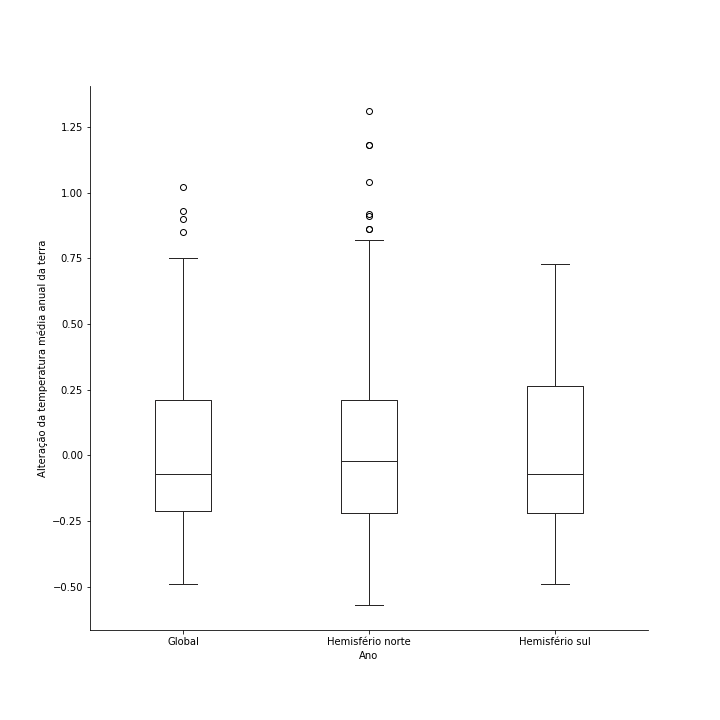
\includegraphics[width = 0.75\textwidth]{boxplot.png}
	\label{fig:A.2}
	\caption{Gráfico de linha mostrando a alteração de temperatura anual da terra pelo tempo.}
\end{figure}

\textbf{\Large Comparação} \par
A pesar dos dois representarem o mesmo conjunto de dados, o objetivo das representações é completamente diferente. O gráfico de linha proporciona uma visualização em que todos os dados são mapeados diretamente, enquanto o boxplot os agrupa e foca em mostrar características dos dados como um conjunto, mas perde todas as individualidades pontuais dos dados. \par
Para determinar algo sobre um momento pontual ou as tendência dos dados, uma visualização de linhas, entre os dois, é a melhor opção. O boxplot vai ter seu 

\newpage
\begin{thebibliography}{9}
	\bibitem{gistemp} 
	GISTEMP Team, 2019: GISS Surface Temperature Analysis (GISTEMP), version 4. NASA Goddard \\
	Institute for Space Studies. Dataset accessed 2019-09-17 at \\\texttt{https://data.giss.nasa.gov/gistemp/}.
	
	\bibitem{latexcompanion} 
	Lenssen, N., G. Schmidt, J. Hansen, M. Menne,A. Persin,R. Ruedy, and D. Zyss, 2019 
	\textit{Improvements in the GISTEMP uncertainty model. J. Geophys. Res. Atmos., 124, no. 12, 6307-6326, doi:10.1029/2018JD029522.}.
\end{thebibliography}

\end{document}